\documentclass{article}
\usepackage[utf8]{inputenc}
\usepackage[papersize={8.5in,11in},margin=0.8in]{geometry}
\usepackage{xcolor}
\usepackage{color, colortbl}
\usepackage{graphicx}
\usepackage{tikz}
\usepackage{amssymb}
\usepackage{amsmath}
\usetikzlibrary{positioning}
\usetikzlibrary{graphs,graphs.standard}


\title{MATH 505 HW 12}
\author{John Caruthers}
\date\today

\begin{document}
\maketitle

\textbf{Section 6.1}
\begin{itemize}
    \item[2.] A sociology quiz contains a true-false question and two multiple-choice questions with possible answers (a), (b), (c), (d). So three total questions, one is true-false, other are multiple choice.
    \begin{itemize}
        \item[a.] In how many possible ways can the test be answered?
        {\color{blue}$2\cdot4\cdot4=32$}
        \item[b.] Verify your answer by drawing a tree diagram and counting the routes.
    \end{itemize}
\end{itemize}
\begin{center}
    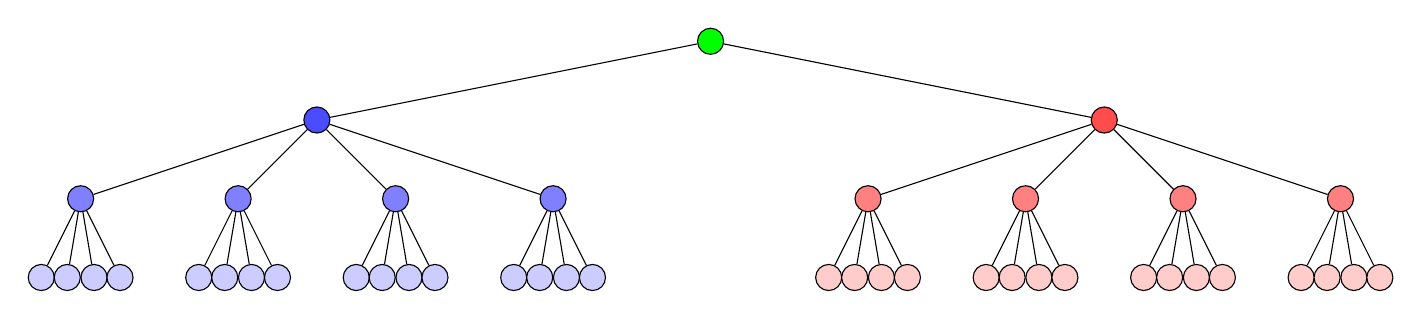
\begin{tikzpicture}[]
      \node(init) at (8,2) [circle, draw=black, fill=green] {};
      \node(t) at (3,1) [circle, draw=black, fill=blue!70] {};
      \node(f) at (13,1) [circle, draw=black, fill=red!70] {};
      
      \node(ta) at (0,0) [circle, draw=black, fill=blue!50] {};
      \node(tb) at (2,0) [circle, draw=black, fill=blue!50] {};
      \node(tc) at (4,0) [circle, draw=black, fill=blue!50] {};
      \node(td) at (6,0) [circle, draw=black, fill=blue!50] {};
      
      \node(fa) at (10,0) [circle, draw=black, fill=red!50] {};
      \node(fb) at (12,0) [circle, draw=black, fill=red!50] {};
      \node(fc) at (14,0) [circle, draw=black, fill=red!50] {};
      \node(fd) at (16,0) [circle, draw=black, fill=red!50] {};
      
      \node(taa) at (-0.5,-1) [circle, draw=black, fill=blue!20] {};
      \node(tab) at (-0.17,-1) [circle, draw=black, fill=blue!20] {};
      \node(tac) at (0.17,-1) [circle, draw=black, fill=blue!20] {};
      \node(tad) at (0.5,-1) [circle, draw=black, fill=blue!20] {};
      
      \node(tba) at (1.5,-1) [circle, draw=black, fill=blue!20] {};
      \node(tbb) at (1.83,-1) [circle, draw=black, fill=blue!20] {};
      \node(tbc) at (2.17,-1) [circle, draw=black, fill=blue!20] {};
      \node(tbd) at (2.5,-1) [circle, draw=black, fill=blue!20] {};
      
      \node(tca) at (3.5,-1) [circle, draw=black, fill=blue!20] {};
      \node(tcb) at (3.83,-1) [circle, draw=black, fill=blue!20] {};
      \node(tcc) at (4.17,-1) [circle, draw=black, fill=blue!20] {};
      \node(tcd) at (4.5,-1) [circle, draw=black, fill=blue!20] {};
      
      \node(tda) at (5.5,-1) [circle, draw=black, fill=blue!20] {};
      \node(tdb) at (5.83,-1) [circle, draw=black, fill=blue!20] {};
      \node(tdc) at (6.17,-1) [circle, draw=black, fill=blue!20] {};
      \node(tdd) at (6.5,-1) [circle, draw=black, fill=blue!20] {};
      
      \node(faa) at (9.5,-1) [circle, draw=black, fill=red!20] {};
      \node(fab) at (9.83,-1) [circle, draw=black, fill=red!20] {};
      \node(fac) at (10.17,-1) [circle, draw=black, fill=red!20] {};
      \node(fad) at (10.5,-1) [circle, draw=black, fill=red!20] {};
      
      \node(fba) at (11.5,-1) [circle, draw=black, fill=red!20] {};
      \node(fbb) at (11.83,-1) [circle, draw=black, fill=red!20] {};
      \node(fbc) at (12.17,-1) [circle, draw=black, fill=red!20] {};
      \node(fbd) at (12.5,-1) [circle, draw=black, fill=red!20] {};
      
      \node(fca) at (13.5,-1) [circle, draw=black, fill=red!20] {};
      \node(fcb) at (13.83,-1) [circle, draw=black, fill=red!20] {};
      \node(fcc) at (14.17,-1) [circle, draw=black, fill=red!20] {};
      \node(fcd) at (14.5,-1) [circle, draw=black, fill=red!20] {};
      
      \node(fda) at (15.5,-1) [circle, draw=black, fill=red!20] {};
      \node(fdb) at (15.83,-1) [circle, draw=black, fill=red!20] {};
      \node(fdc) at (16.17,-1) [circle, draw=black, fill=red!20] {};
      \node(fdd) at (16.5,-1) [circle, draw=black, fill=red!20] {};
      
      \path[-] (init) edge (t);
      \path[-] (init) edge (f);
      
      \path[-] (t) edge (ta);
      \path[-] (t) edge (tb);
      \path[-] (t) edge (tc);
      \path[-] (t) edge (td);
      
      \path[-] (ta) edge (taa);
      \path[-] (ta) edge (tab);
      \path[-] (ta) edge (tac);
      \path[-] (ta) edge (tad);
      
      \path[-] (tb) edge (tba);
      \path[-] (tb) edge (tbb);
      \path[-] (tb) edge (tbc);
      \path[-] (tb) edge (tbd);
      
      \path[-] (tc) edge (tca);
      \path[-] (tc) edge (tcb);
      \path[-] (tc) edge (tcc);
      \path[-] (tc) edge (tcd);
      
      \path[-] (td) edge (tda);
      \path[-] (td) edge (tdb);
      \path[-] (td) edge (tdc);
      \path[-] (td) edge (tdd);
      
      \path[-] (f) edge (fa);
      \path[-] (f) edge (fb);
      \path[-] (f) edge (fc);
      \path[-] (f) edge (fd);
      
      \path[-] (fa) edge (faa);
      \path[-] (fa) edge (fab);
      \path[-] (fa) edge (fac);
      \path[-] (fa) edge (fad);
      
      \path[-] (fb) edge (fba);
      \path[-] (fb) edge (fbb);
      \path[-] (fb) edge (fbc);
      \path[-] (fb) edge (fbd);
      
      \path[-] (fc) edge (fca);
      \path[-] (fc) edge (fcb);
      \path[-] (fc) edge (fcc);
      \path[-] (fc) edge (fcd);
      
      \path[-] (fd) edge (fda);
      \path[-] (fd) edge (fdb);
      \path[-] (fd) edge (fdc);
      \path[-] (fd) edge (fdd);
    \end{tikzpicture}
\end{center}
\begin{itemize}
    \item[4.] Kate wants to buy an automobile. She has a choice of 2 body styles (2-door or 4-door), 2 types of transmissions (auto or manual), and 4 colors (green, red, black, or blue).  In how many ways can she select an automobile?\\ {\color{blue} $2\cdot2\cdot4=16$}
    \item[8.] Compute the following factorial numbers without using a calculator.
    \begin{itemize}
        \item[a.] $4!$ {\color{blue}= $4\cdot3\cdot2\cdot1=24$}
        \item[b.] $7!$ {\color{blue}= $7\cdot6\cdot5\cdot4\cdot3\cdot2\cdot1=5040$}
        \item[c.] $0!$ {\color{blue}= $1$}
        \item[d.] $1!$ {\color{blue}= $1$}
    \end{itemize}
    \item[12.] Evaluate each of the following permutation numbers.
    \begin{itemize}
        \item[b.] $P(6,5)$ {\color{blue}= $\frac{6!}{(6-5)!} = \frac{6!}{1!}=6!=720$}
        \item[d.] $P(9,2)$ {\color{blue}= $\frac{9!}{(9-2)!} = \frac{9!}{7!}=9\cdot8=72$}
        \item[f.] $P(8,7)$ {\color{blue}= $\frac{8!}{(8-7)!} = \frac{8!}{1!}=8!=40320$}
    \end{itemize}
    \item[15.] Write a simple expression for each of the following.
    \begin{itemize}
        \item[a.] $P(r,1)$ {\color{blue}= $\frac{r!}{(r-1)!}=r$}
        \item[b.] $P(k,2)$ {\color{blue}= $\frac{k!}{(k-2)!}=k\cdot(k-1)=k^2-k$}
        \item[c.] $P(r,r-1)$ {\color{blue}= $\frac{r!}{(r-(r-1))!}=\frac{r!}{(r-r+1)!}=\frac{r!}{1!}=r!$}
    \end{itemize}
\end{itemize}
\textbf{Section 6.2}
\begin{itemize}
    \item[2.] Compute the following combination numbers
    \begin{itemize} 
        \item[a.] $C(4,2)$ {\color{blue}= $\frac{4!}{2!(4-2)!}=\frac{4!}{2!\cdot2!}=\frac{4\cdot3}{2!}=6$}
        \item[b.] $C(7,5)$ {\color{blue}= $\frac{7!}{2!(7-2)!}=\frac{7!}{2!\cdot5!}=\frac{7\cdot6}{2!}=21$}
        \item[c.] $C(5,5)$ {\color{blue}= $\frac{5!}{5!(5-5)!}=\frac{5!}{5!\cdot1}=1$}
    \end{itemize}
    \item[3.] If $A$ is a set with $n$ elements, where $n$ is a positive integer, how many subsets of $A$ have:
    \begin{itemize}
        \item[a.] no elements: {\color{blue} 1 since every set contains an empty subset}
        \item[b.] exactly 1 element: {\color{blue} $C(n,1)=\frac{n!}{1(n-1)!}=n$}
        \item[c.] exactly $n-1$ elements: {\color{blue} $C(n,n-1)=\frac{n!}{(n-1)!(n-(n-1))!}=\frac{n!}{1\cdot(n-1)!}=n$}
        \item[d.] $n$ elements: {\color{blue} $C(n,n)=\frac{n!}{n!(n-n)!}=\frac{n!}{1\cdot n!}=1$}
    \end{itemize}
    \item[6.] Recall that a standard deck of cards has 52 cards.  How many 5-card poker hands have:
    \begin{itemize}
        \item[a.] 4 queens: A 5-card poker hand with 4 queens has all the possible queens AND one of any other non-queen card.  4 queens is $C(4,4)$ and any one of the other non-queens is $C(48,1)$.
        \begin{align}
            C(4,4)&={\color{blue}1}\nonumber\\
            C(48,1)&=\frac{48!}{1!\cdot(48-1)!}=\frac{48!}{1\cdot47!}={\color{blue}48}\nonumber
        \end{align}
        {\color{blue} Using the multiplication rule, there are $1\cdot48=48$ hands containing exactly 4 queens.}
        \item[b.] 5 clubs: A 5-card poker hand with 5 clubs has only clubs and 0 of any other card.  Since there are 13 clubs, 4 clubs is $C(13,5)$.  There are 39 non-clubs and 0 of any other card is $C(39,0)$.
        \begin{align}
            C(13,5)&=\frac{13!}{5!(13-5)!}=\frac{13!}{5!\cdot8!}={\color{blue}1287}\nonumber\\
            C(39,0)&=\frac{39!}{0!\cdot39!}={\color{blue}1}\nonumber
        \end{align}
        {\color{blue} Using the multiplication rule, there are $1287\cdot1=1287$ hands containing exactly 5 clubs.}
        \item[c.] 3 queens and 2 jacks: A 5-card poker hand with 3 queens AND 2 jacks. 3 queens is $C(4,3)$ since there are only 4 queens total.  2 jacks is $C(4,2)$ since there are only 4 jacks total.
        \begin{align}
            C(4,3)&=\frac{4!}{3!(4-3)!}=\frac{4!}{3!\cdot1!}={\color{blue}4}\nonumber\\
            C(4,2)&=\frac{4!}{2!(4-2)!}=\frac{4!}{2!\cdot2!}={\color{blue}6}\nonumber
        \end{align}
        {\color{blue} Using the multiplication rule, there are $4\cdot6=24$ hands containing 3 queens and 2 jacks.}
        \item[d.] No hearts: A 5-card poker hand with no hearts is C(39,5) since out of 52 cards, 39 are not hearts and need to calculate how many unique subsets of length 5 exist. There are 0 of any other card which is {\color{blue}1}.
        \begin{align}
            C(39,5)&=\frac{39!}{5!(39-5)!}=\frac{39!}{5!\cdot34!}={\color{blue}575757}\nonumber
        \end{align}
        {\color{blue} Using the multiplication rule, there are $575757\cdot1=575757$ hands containing no hearts.}
    \end{itemize}
    \item[10.] A package of jellybeans has 15 green jellybeans and 11 red jellybeans.  In how many ways can you choose a handful of 5 jellybeans in which there are:
    \begin{itemize}
        \item[a.] 2 green and 3 red jellybeans: 2 green jellybeans is $C(15,2)$ and 3 red jellybeans is $C(11,3)$.
        \begin{align}
            C(15,2)&=\frac{15!}{2!(15-2)!}=\frac{15!}{2!\cdot13!}={\color{blue}105}\nonumber\\
            C(11,3)&=\frac{11!}{3!(11-3)!}=\frac{11!}{3!\cdot8!}={\color{blue}165}\nonumber
        \end{align}
        {\color{blue} There are $105\cdot165=17325$ ways to pick 2 green and 3 red jellybeans.}
        \item[b.] At least 3 red jellybeans: This is 3, 4 and 5 red jellybeans; the combination of $C(11,3), C(11,4),$ and $C(11,5)$. From the previous problem, $C(11,3)={\color{blue}165}$. Next just need to calculate $C(11,4)$ and $C(11,5)$.
        \begin{align}
            C(11,4)&=\frac{11!}{4!(11-4)!}=\frac{11!}{4!\cdot7!}={\color{blue}330}\nonumber\\
            C(11,5)&=\frac{11!}{5!(11-5)!}=\frac{11!}{5!6!}={\color{blue}462}\nonumber
        \end{align}
        {\color{blue}Using the multiplication rule, there are $165\cdot330\cdot462=25155900$  ways to pick subsets of 5 containing at least 3 red jellybeans.}
    \end{itemize}
\end{itemize}
\textbf{Section 6.3}
\begin{itemize}
    \item[1.] Let $S$ be a set with 8 elements.  Use Pascals triangle to answer the following questions.
    The 8th row of Pascals triangle is {\color{olive}1 8 28 56 70 56 28 8 1}. Use this to answer the questions below.  For example, 2 elements would correspond to the 2nd row (Pascals triangle rows and columns start at 0).
    \begin{itemize}
        \item[a.] How many subsets of $S$ have exactly 2 elements? {\color{blue}28}
        \item[b.] How many subsets of $S$ have exactly 3 elements? {\color{blue}56}
        \item[c.] How many subsets of $S$ have exactly 4 elements?
        {\color{blue}70}
        \item[d.] How many subsets of $S$ have exactly 5 elements?
        {\color{blue}56}
        \item[e.] How many subsets of $S$ are there together? {\color{blue}$1+8+28+56+70+56+28+8+1=2^8= 256$}
    \end{itemize}
    \item[5.] How many arrangements of 0's and 1's are there with: These are the total number of combinations which can be solved using binomial coefficients.   $x^ry^{n-r}$ where $r$ is the number of $0's$ and $n$ is the total number of $0's$ and $1's$.
    \begin{itemize}
        \item[a.] four 0's and ten 1's {\color{blue} $x^4y^{10}=1001$}
        \item[b.] five 0's and nine 1's {\color{blue} $x^5y^9=2002$}
        \item[c.] six 0's and eight 1's {\color{blue} $x^6y^8=3003$}
    \end{itemize}
    \item[7.] In the expansion of $(x+y)^{14}$, determine the coefficient:
    Using Theorem 3, the coefficient of $x^ry^{n-r}$ in the expansion of $(x+y)^n$ is $C(n,r)$.
    \begin{itemize}
        \item[a.] $x^4y^{10}$ {\color{blue}1001}
        \item[b.] $x^5y^9$ {\color{blue}2002}
        \item[c.] $x^6y^8$ {\color{blue}3003}
    \end{itemize}
\end{itemize}
\end{document}
 
